\chapter{FUNDAMENTAÇÃO TEÓRICA}
Neste capítulo, são apresentados os principais conceitos e fundamentos necessários para a compreensão, 
entendimento e progresso deste trabalho.

\section{Séries Temporais}
    Muitas pessoas, em algum momento, já imaginaram como seria prever o futuro e ter acesso a informações sobre eventos 
    ou situações de suas vidas. Essa curiosidade reflete um desejo universal, mas também uma necessidade presente em 
    diversas áreas, como na gestão governamental, no setor financeiro e em contextos sociais. Nesse cenário, surge o 
    conceito de Série Temporal, definido como um conjunto de observações organizadas sequencialmente no tempo, 
    representadas por \( x_t \), com cada valor correspondente a um instante específico \(t\)~\cite{box2015}. O estudo de 
    Séries Temporais permite não apenas compreender as características de fenômenos que evoluem ao longo do tempo, mas 
    também desenvolver e ajustar modelos estatísticos capazes de explicar ou prever o comportamento dos dados 
    observados.
    
    De acordo com~\citeonline{brockwell2002}, séries temporais podem ser classificadas 
    discretas e continuas, uma série temporal é discreta quando o conjunto \( t_0 \) de tempos em que as observações 
    são feitas é um conjunto discreto, como o caso de observações que são realizadas em um determinado intervalo de 
    tempo fixo. Sendo representada por:
    \begin{equation}
        T = \{t_1, \dots, t_n\}, \quad \{X_t : t \in T\}
    \end{equation}
    
    
    E seríes temporais continuas quando suas observações são obtidas continuamente no tempo. Sendo expressa por: 
    \begin{equation}
        T = [t_1, t_2], \quad \{X(t) : t \in T\}
    \end{equation}
        
    \subsection{Estacionariedade}
        A estacionariedade refere-se ao comportamento dos valores de uma série temporal ao longo do tempo. Uma série é 
        classificada como estacionária quando seus dados flutuam de maneira aleatória em torno de uma média fixa, mantendo-se em 
        um estado de equilíbrio ao longo do período analisado. Contudo, na prática, muitas séries temporais do cotidiano não 
        apresentam essa característica, exibindo tendências, sazonalidades ou outras formas de variação que indicam a presença de 
        não estacionariedade~\cite{morettin2018}.

    \subsubsection{Teste de Estacionariedade}
        A maioria dos métodos comuns de análise estatística de séries temporais parte do princípio de que as 
        séries a serem analisadas são estacionárias. Para verificar essa condição, é necessário aplicar 
        testes de estacionariedade. Um dos mais conhecidos e utilizados é o teste de Dickey-Fuller Aumentado, 
        que tem como objetivo identificar a presença de raízes unitárias nos operadores de 
        retardos\footnote{Raízes dos operadores de retardos vêm da equação característica de um sistema. 
        Em séries temporais, elas determinam a estacionariedade.}~\cite{costa2019}

        As hipóteses nula e alternativa do teste Dickey-Fuller Aumentado são:

        \begin{center}
            \(H_0\) : a série possui raiz unitária

            \(H_1\) : a série não possui raiz unitária
        \end{center}

        Caso a série tenha raiz unitária, ela não é estacionária; se não possuir raiz unitária, a série é estacionária.
    \subsection{Decomposição}

        De acordo com \citeonline{costa2019}, a análise inicial de uma série temporal se beneficia 
        significativamente do uso de gráficos que exibem os dados em ordem cronológica, pois essa abordagem 
        facilita a identificação de padrões e características inerentes, tais como tendência, sazonalidade, 
        ciclicidade e ruído (erro aleatório). Além disso, \citeonline{correa2024} esclarece o significado 
        desses padrões, contribuindo para uma compreensão mais aprofundada dos comportamentos presentes nas 
        séries.
        
        A tendência ($\mu_t$) representa o padrão de variação de uma grandeza ao longo do tempo. Em termos gerais, ela indica se 
        uma série temporal segue um crescimento ou um declínio de forma consistente. Séries temporais que exibem esse comportamento 
        são classificadas como não estacionárias.

        
        A ciclicidade ($\psi_t$) refere-se a variações nos dados que ocorrem em intervalos regulares, com uma duração superior a um 
        ano. Esses ciclos podem estar associados a fatores econômicos, políticos ou sociais, manifestando-se de forma recorrente ao 
        longo do tempo.     
        
        A sazonalidade ($\gamma_t$) é uma variação periódica que se repete em intervalos regulares, mantendo a mesma frequência e 
        intensidade, ocorrendo em um intervalo de tempo menor que um ano. Esse comportamento pode ser observado em 
        vendas durante datas comemorativas anuais, como Páscoa, Natal e São João, além de em padrões climáticos.
        
        O ruído ($\epsilon_t$) representa a variabilidade imprevisível em uma série temporal, correspondendo a flutuações que não 
        podem ser explicadas por outros componentes. Além disso, ele atua como uma fonte de erro nas previsões, afetando a precisão 
        dos modelos.


    \subsection{Modelos}
        \citeonline{morettin2018} afirmam que modelos probabilísticos ou estocásticos podem ser construídos no 
        domínio temporal ou de frequências. Além disso, esses modelos devem ser simples e conter um número 
        reduzido de parâmetros.~\citeonline{morettin2018} também destacam a existência de diferentes modelos 
        que utilizam distintos métodos computacionais para calcular a mesma estimativa, especificamente a 
        previsão de mínimos~\footnote{O metódo dos minímos quadrados é uma técnica que busca encontrar o 
        gráfico de melhor ajuste para um conjunto de amostras de dados~\cite{miyasaki2010}.} de um valor 
        futuro com base em combinações lineares de valores passados.

        \subsubsection{ARIMA}
            O modelo ARIMA (Autoregressive Integrated Moving Average) foi criado nos anos 1970 por George Box
            e Gwilym Jenkins, visando descrever as mudanças nas séries temporais utilizando a combinação de três
            componentes principais, conhecidos também como filtros \((p, d, q)\), sendo eles:
            \begin{itemize}
                \item Autoregressão \emph{(AR)};
                \item Integração \emph{(I)};
                \item Média Móvel \emph{(MA)};
            \end{itemize}

            O componente \emph{AR}, ou filtro \(p\), tange à dependência das observações atuais em relação às observações
            passadasm, visto que ele toma como base a intuição de que o passado prediz o futuro. Com isso, ele 
            pressupõe um processo de série temporal no qual o valor em um ponto no tempo \(t\) é uma função
            dos valores da série em pontos anteriores no tempo. É dada por~\eqref{eq:modelo_ar}.
            
            \begin{equation}
                y_t = \phi_0 + \phi_1 y_{t-1} + \phi_2 y_{t-2} + \ldots + \phi_p y_{t-p} + e_t
                \label{eq:modelo_ar}
            \end{equation}
            
            \(y_t\) é o valor da série temporal no tempo \(t\). Sendo a variável dependente, a qual queremos
            prever.~\(\phi_0\) constante que representa o termo intercepto. 
            \(\phi_1, \phi_2, \ldots, \phi_p \) são os coeficientes do modelo que
            indicam a influência dos valores passados \(y_{t-1}, y_{t-2}, \ldots, y_{t-p}\) no valor atual 
            \(y_t\) da série. \(y_{t-1}, y_{t-2}, \ldots, y_{t-p}\) são defasagens da variável \(y_t\), ou seja,
            valores passados da série. Sendo que a ordem \(p\) indica até quantos períodos anteriores são 
            considerados para prever o valor atual. E \(e_t\) é um termo de erro que varia com o tempo, pressupõe-se 
            que esse termo de erro possui uma variância constante e uma média 0.

            O componente \emph{MA}, ou filtro \(q\), baseia-se em um processo no qual o valor em cada 
            instante é determinado por uma função dos termos de ``erro'' do passado recente, tratados como 
            independentes entre si. De forma similar a um modelo de regressão, esse componente modela a 
            relação entre as observações atuais e os erros anteriores~\cite{nielsen2021analise,correa2024}.
            Ele é definido pela equação~\eqref{eq:modelo_ma}, onde \(y_t\) representa o valor a ser previsto e 
            \( \theta_1, \theta_2, \ldots, \theta_q \) são os coeficientes da média móvel, os quais ponderam 
            os termos de erro presentes e passados~\cite{nielsen2021analise}.

            \begin{equation}
                y_t = \mu + e_t + \theta_1 e_{t-1} + \theta_2 e_{t-2} + \ldots + \theta_q e_{t-q}
                \label{eq:modelo_ma}
            \end{equation}

            Por fim, o componente \emph{I} ou filtro \(d\), refere-se à aplicação de diferenciação aos dados 
            com o intuito de torná-los estacionários. Em termos práticos, isso significa subtrair cada a
            observação de sua predecessora, removendo assim tendências e sazonalidades~\cite{nielsen2021analise,correa2024}. 
            Essa operação é descrita pela equação~\eqref{eq:modelo_i}, onde \(y'_t\) epresenta a diferença 
            entre os valores consecutivos da série temporal, \(y_t\) é o valor da série no tempo \(t\) e \(y_{t-1}\)
            corresponde ao período imediatamente anterior. Em essência, a diferenciação converte uma série 
            temporal de valores em uma série de variações, facilitando a análise das mudanças ao longo do 
            tempo.
            
            \begin{equation}
                y'_t = y_t - y_{t-1}
                \label{eq:modelo_i}
            \end{equation}  

            O ARIMA combina os modelos \emph{AR} e \emph{MA}, criando o modelo \emph{ARMA}, por fim adicionando 
            a diferenciação \emph{I}.~\citeonline{morettin2018} recomenda que, antes da modelagem, seja realizado um teste
            de estacionariedade na série a ser analisada. Se a série for estacionária, o filtro \(d\) será 0, 
            resultando em um modelo \emph{ARMA}(p, 0, q). Todavia, pode-se utilizar o modelo \emph{ARMA}
            expresso na equação~\eqref{eq:modelo_arma}.  Caso a série não seja estacionária, torna-se necessário aplicar 
            diferenciações, conforme a equação \eqref{eq:modelo_i}, até que a série se estabilize e o modelo \emph{ARMA} possa 
            ser empregado.

            
            \begin{equation}
                y_t = \phi_0 + \sum (\phi_i r_{t-i}) + e_t - \sum (\theta_i e_{t-i}) 
                \label{eq:modelo_arma}
            \end{equation}
        
        \subsubsection{SARIMA}
            Muitas séries temporais exibem padrões recorrentes que se repetem em intervalos regulares. O modelo 
            ARIMA sazonal (SARIMA) assume uma estrutura multiplicativa para essa sazonalidade, possibilitando 
            que o comportamento sazonal seja modelado como um processo ARIMA à parte. Assim, o modelo pode ser 
            expresso pela notação
            \[
            \text{ARIMA}(p,d,q) \times (P,D,Q)_m,
            \]
            onde \( m \) indica o número de intervalos de tempo em cada ciclo sazonal~\cite{nielsen2021analise}.

\section{Redes Neurais}
%Falar brevemente
    Analisando o cerebro, percebeu-se a constituição complexa, não linear e paralela dele, sendo composto por 10 bilhos de neurônios.
    Cada neurônio conectado, em média, a outros 10 bilhões de neurônios, formando uma vasta e sofistiada rede~\cite{haykin2009neural}.

    Em uma rede neural, a comunicação é realizada através de sinais eletroquímicos, e esses sinais são transmitidos 
    e processados através dos componentes presentes em sua estrutura. Os componentes presentes na estrutura de um neurônio 
    são exibidos na Figura \ref{fig:neuronio_biologico}:
    \begin{figure}[!htb]
        \centering
        \caption{Neurônio Biológico.}
        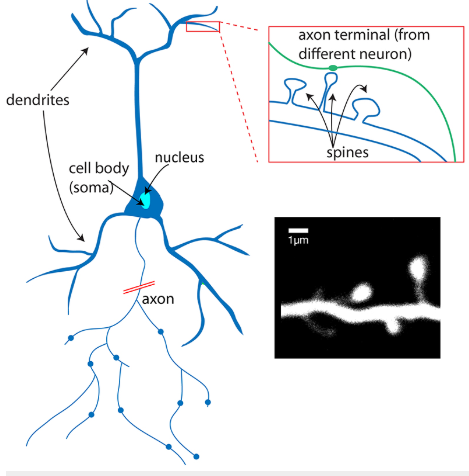
\includegraphics[scale=0.5]{celula-piramidial.png}\\
        {\footnotesize Fonte: The University Of Queensland.}\
        \label{fig:neuronio_biologico}
    \end{figure}
    
    \begin{itemize}
        \item \textbf{Corpo Celular ou Soma: }responsável por integrar os sinais recebidos de outros neurônios;
        \item \textbf{Dendritos: }responsáveis por receber informações transmitidas por outros neurônios. 
        São consideradas as zonas receptivas;
        \item \textbf{Axônio: }responsável por transmitir as informações para outros neurônio, também chamado de linha de 
        transmissão;
    \end{itemize}

    Quando o conjunto de sinais recebidos é suficientemente forte para ativar o neurônio, este gera um impulso elétrico 
    que percorre seu axônio. Esse sinal eletroquímico coordena e organiza a atividade neuronal, permitindo ao cérebro realizar 
    diversas formas de processamento de maneira extremamente eficiente, muitas vezes mais rápida do que os computadores digitais 
    convencionais~\cite{haykin2009neural}. Ao entender de que forma o cerebro humano processa informações, cientistas buscaram 
    reproduzir seu funcionamento de forma artificial.
    
    Com isso, surgiram as Redes Neurais Artificiais (RNA's), que tenta mimetizar o sistema nervoso humano. RNA's são capazes de
    assimilar e reter conhecimento, possuíndo um alto grau de paralelsimo e extremamente conectada. As RNA's são utilizadas para
    desempenhar a mesma função após o treinamento. Sendo seu elemento constituinte chamado de neurônio artificial~\cite{ulinick2019}.

    De acordo com \citeonline{haykin2009neural}, um neurônio é uma unidade de processamento de informação que é fundamental para a operação de um
    rede neural. Na Figura \ref{fig:fluxo-perceptron} é ilustrado os componentes básicos da arquitetura mais simples de uma rede neural.
    \begin{figure}[!htb]
        \centering
        \caption{Neurônio Artificial (Perceptron).}
        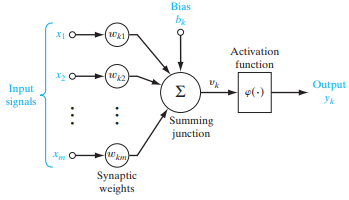
\includegraphics[scale=0.8]{fluxo-perceptron.png}\\
        {\footnotesize Fonte: Haykin (2009).}\
        \label{fig:fluxo-perceptron}
    \end{figure}
    
    \begin{itemize}
        \item \textbf{Camada de Entrada: }Responsável por receber as informações do ambiente 
        externo e transmiti-las ao restante da rede para processamento.
        \item \textbf{Sinapses: }Representam as conexões entre os neurônios, simuladas por pesos 
        \( w_1, w_2, \dots, w_n \), que determinam se o sinal terá um efeito estimulante (excitador) ou 
        inibidor.
        \item \textbf{Bias: }É um valor adicional que ajusta a ativação do neurônio, permitindo que ele 
        se "ajuste" de forma mais flexível. O viés pode ser positivo ou negativo e ajuda a rede a decidir 
        quando ativar ou não o neurônio, independentemente das entradas. Ele atua como uma espécie de 
        "ajuste fino", permitindo que a rede aprenda melhor a partir dos dados.
        \item \textbf{Somador: }Mecanismo que agrega todas as entradas, considerando seus respectivos 
        pesos, para gerar um valor combinado.
        \item \textbf{Função de ativação: }Limita a amplitude do sinal de saída a um intervalo finito, 
        determinando se o neurônio será ativado com base na soma ponderada das entradas.
        \item \textbf{Camada de Saída: }Fornece o resultado final do processamento do neurônio, 
        representando a resposta da rede ao estímulo recebido.
    
    \end{itemize}
    % \subsection{Histórico}
    %     As redes neurais são frequentemente consideradas um complemento à computação tradicional. Curiosamente, 
    %     John von Neumann, amplamente reconhecido como o pai da computação moderna devido à sua proposta da arquitetura 
    %     que possibilitou a criação do computador de programa armazenado, demonstrava grande interesse em modelar o 
    %     funcionamento do cérebro humano. Esse interesse levantou debates entre pesquisadores sobre a possível interação 
    %     entre as ideias de von Neumann e os primórdios das redes neurais. Alguns estudiosos destacam indícios que 
    %     sugerem a visão de von Neumann sobre as direções futuras do desenvolvimento dos computadores~\cite{Fausett1994}.

    %     Neste capítulo, serão destacados alguns marcos significativos que tiveram um papel fundamental no avanço e
    %     desenvolvimento da área de redes neurais.

    %     \subsubsection{Perceptrons}
            
    %         Em 1958, o psicólogo Frank Rosenblatt publicou um artigo que, pela primeira vez, descreveu de forma 
    %         algorítmica o funcionamento de um modelo de rede neural para aprendizagem supervisioanda. Essa 
    %         publicação inspirou inúmeros pesquisadores a direcionarem seus esforços para estudos sobre redes neurais, 
    %         explorando diversos aspectos dessa temática ao longo das décadas de 1960 e 1970~\cite{haykin2009neural}.

    %         \begin{figure}[!htb]
    %             \centering
    %             \caption{Fluxo do perceptron.}
    %             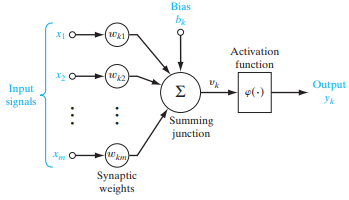
\includegraphics[scale=0.8]{fluxo-perceptron.png}\\
    %             {\footnotesize Fonte: Haykin (2009).}\
    %             \label{fig:fluxo-perceptron}
    %         \end{figure}

    %         Como apresentado na Figura~\ref{fig:fluxo-perceptron}, o perceptron consiste de um único neurônio com 
    %         pesos sinápticos ajustáveis e um viés. Ele possui uma camada de entrada (a retina) conectada aos pesos e 
    %         uma camada de saída. Seu funcionamento baseia-se em um combinador linear seguido por uma função de 
    %         ativação que realiza uma função linear. Esse nó somador (o neurônio) calcula uma combinação linear das 
    %         entradas aplicadas às suas sinapses, além de incorporar um viés aplicado externamente que ajusta a posição
    %         da função de ativação. O resultado dessa soma é passado à função de ativação, que produz uma saída de +1 
    %         se a entrada for positiva, ou -1, se for negativa. 
            
    %         O perceptron é um classificador binário, pois resolve apenas problemas de classificação de padrões 
    %         linearmente separáveis, ou seja, é capaz de lidar exclusivamente com problemas nos quais duas classes 
    %         podem ser separadas por uma linha em um hiperplano~\cite{haykin2009neural}. 


        % \subsubsection{Adaline}

        %     Em 1960, Bernard Widrow e Marcian Hoff desenvolveram uma regra de aprendizagem denominada "Regra Delta", 
        %     também conhecida como Least Mean Squares (LMS) ou método do Gradiente Descendente. Com base nessa regra, 
        %     foi criada uma rede neural com a mesma estrutura do Perceptron, composta por uma camada de entrada, uma 
        %     camada de saída e um único neurônio. A diferença principal reside na regra de aprendizado empregada para 
        %     o ajuste dos pesos, enquanto o Perceptron ajusta os pesos com base na saída binária da rede, essa rede
        %     utiliza a diferença entre o previsto e real e aplica o gradiente descendente para reduzir o erro.
            
        %     A Regra Delta, que tem como finalidade ajustar os pesos do neurônio, busca minimizar a diferença entre a 
        %     saída desejada e a resposta obtida a partir da combinação linear de todas as amostras. Utilizando a 
        %     minimização do erro quadrático médio entre os valores previstos e reais, o método opera dentro de um 
        %     contexto de aprendizagem supervisionada, onde há uma saída esperada previamente definida. O algoritmo 
        %     ajusta iterativamente o vetor de pesos \( w\) atribuído à rede, com o objetivo de determinar um 
        %     \( w^{*} \) ótimo tal que o erro quadrático \({E(w{*})}\), calculado sobre todo o conjunto de amostras, 
        %     seja minimizado.

        %     Essa rede neural foi projetada para aplicações em sistemas de chaveamento de circuitos telefônicos e 
        %     ficou conhecida como Adaline (Adaptive Linear Neuron). A Adaline foi uma das primeiras redes neurais 
        %     implementadas em contextos industriais, marcando um avanço significativo na aplicação de tecnologias 
        %     baseadas em inteligência artificial. Além disso, a regra de aprendizagem Widrow-Hoff para uma rede neural 
        %     de apenas uma camada foi o percursor da regra de Backpropagation para múltiplas camadas~\cite{Fausett1994,silva2010}
                
    \subsection{Processo de Treinamento}
        Sistemas de aprendizado de máquina podem ser categorizados de acordo com o tipo de treinamento que
        eles recebem. O aprendizado supervisionado ocorre quando o modelo é treinado por meio de exemplos explícitos. 
        Em contrapartida, no aprendizado não supervisionado, não há a definição de exemplos explícitos para orientar o 
        modelo. Além disso, existem diversas boas práticas para garantir que o modelo consiga realizar um aprendizado satisfatório 
        e métricas para avalia-lo
         
        \subsubsection{Aprendizado Supervisionado e Não Supervisionado}  
        %Falar de forma breve o que é o aprendizado supervisionado e seus tipos
            No aprendizado supervisionado, o modelo é treinado com pares de dados \((x,y)\), onde \(x\) representa 
            os dados de entrada e \(y\) o valor esperado (ou rótulo). Durante o treinamento, o modelo compara as 
            previsões feitas com os valores reais utilizando uma função de perda, que mede o erro. Em seguida, 
            seus parâmetros são ajustados iterativamente, geralmente por meio de métodos como o gradiente descendente, 
            para minimizar esse erro e melhorar a precisão das previsões~\cite{ulinick2019}.
            
            No aprendizado não supervisionado, o modelo não recebe o par de dados \((x,y)\), mas apenas as entradas 
            \(x\). A partir disso, ele busca identificar padrões, estruturas ou associações presentes nos dados, 
            ajustando os pesos de acordo com o objetivo do método utilizado~\cite{ulinick2019}.

        
        \subsubsection{Pre-Processamento dos Dados}
            Antes de treinar um modelo com algoritmos de aprendizado de máquina, é imprescindível realizar o pré-processamento 
            dos dados. Esse processo assegura que os dados estejam padronizados, consistentes e adequados, permitindo que os 
            modelos alcancem um desempenho superior e resultados confiáveis nas métricas de avaliação. Para isso, são utilizadas 
            técnicas que evitam problemas como dados ausentes, inconsistências, valores conflitantes e incongruentes. Essas 
            técnicas são geralmente divididas em quatro categorias principais: limpeza, integração, transformação e redução de 
            dados~\cite{silva2021, oliveira2024}.

            \subsubsubsection{Limpeza de Dados}
                Um problema comum em conjuntos de dados (\emph{datasets}) é a presença de valores faltantes (ou nulos), que 
                podem ocorrer devido a diferentes fatores. Esses fatores incluem registros manuais realizados de forma 
                inadequada, falhas em sistemas de extração, transformação e carregamento de dados (\emph{ETL}) ou até mesmo 
                problemas em sensores de dispositivos autônomos. A presença de valores faltantes compromete tanto a qualidade 
                dos dados quanto o desempenho do treinamento de modelos de \emph{machine learning}, caso não seja tratada 
                adequadamente.~\citeonline{sivakumar2017} apresentam algumas abordagens eficazes para lidar com essa 
                problemática, como:

                \begin{itemize}
                    \item Exclusão de linhas do \emph{dataset} que contenham valores faltantes.
                    \item Preenchimento dos valores ausentes utilizando métricas estatísticas, como a média ou mediana, 
                    para gerar estimativas aproximadas que mantenham a coerência do conjunto de dados.
                \end{itemize}
                
            \subsubsubsection{Integração de Dados}
                É o processo de combinar dados provenientes de diversas fontes, ecossistemas e tecnologias, de maneira adequada 
                e coerente. Durante esse processo de integração, podem surgir problemas, como inconsistências nos dados e 
                redundâncias no conjunto de dados gerado~\cite{sivakumar2017, silva2021, oliveira2024}.

            \subsubsubsection{Transformação de Dados}
                Nesse estágio, os dados são transformados em formatos adequados para utilização no modelo. 
                \citeonline{sivakumar2017} e \citeonline{oliveira2024} definem algumas atividades executadas nesta 
                etapa:

                \begin{itemize} 
                    \item Uso de normalização para ajustar os valores dos dados a uma escala comum, permitindo fácil comparação entre 
                    diferentes atributos. 
                    \item Eliminação de ruídos com técnicas de suavização. 
                    \item Aplicação de técnicas de agregação para resumir dados complexos e detalhados. 
                    \item Generalização de valores específicos em categorias mais amplas, como, por exemplo, a generalização de 
                    faixas etárias. 
                \end{itemize}

            \subsubsubsection{Redução de Dados}
                Nessa etapa, são utilizadas metodos para reduzir o volume de dados que serão analisados, visando maior velocidade
                de processamento e melhora na eficiência do processo, mas sem comprometer a qualidade e integridade dos dados 
                originais.~\citeonline{sivakumar2017} indicam algumas estrategias, sendo elas:
                \begin{itemize}
                    \item Redução de dimensionalidade do \emph{dataset}, removendo atributos que não melhoram a perfomance do 
                    modelo.
                    \item Utilização de operações de agregação de dados para resumo de informações.
                    \item Utilização de técnicas de \emph{encoding} para compactação de dados.
                \end{itemize}

        \subsubsection{Overfitting e Undefitting}
            Ao construir modelos de redes neurais, diversos desafios podem surgir, sendo dois dos mais comuns: o 
            \emph{Overfitting} e o \emph{Underfitting}. O \emph{Overfitting} ocorre quando o modelo aprende tão 
            bem os padrões dos dados de treinamento que sua capacidade de generalização para novos dados é 
            comprometida. Isso acontece porque o modelo não apenas captura as características relevantes dos dados, 
            mas também absorve ruídos e padrões específicos do conjunto de treinamento~\cite{montesinos2022}. 
            Como consequência, ao ser exposto a novos exemplos, seja do conjunto de teste ou de outros conjuntos de 
            dados inéditos, o modelo tende a aplicar regras memorizadas, em vez de identificar padrões generalizáveis. 
            Isso compromete sua capacidade de inferir corretamente a partir de dados não vistos, resultando em um 
            desempenho insatisfatório.

            Por outro lado, o \emph{Underfitting} ocorre quando o modelo é excessivamente simples, muitas vezes 
            devido à utilização de poucas variáveis de entrada. Isso impede que o modelo represente adequadamente 
            os padrões predominantes no \emph{dataset} e capture as características essenciais das amostras, 
            resultando em um desempenho insatisfatório já durante o treinamento. Além disso, esse problema também 
            pode surgir quando o conjunto de dados de treinamento é muito pequeno ou pouco representativo da 
            população, comprometendo ainda mais a capacidade de aprendizagem do modelo~\cite{montesinos2022}.
            
        

        \subsubsection{Técnicas de Validação}
        %Falar o que é, porque foi criada e modo de uso
        A validação é uma etapa crucial para avaliar a capacidade preditiva de um modelo de 
        \emph{machine learning}, além de ser fundamental para o ajuste de seus hiperparâmetros.
        \subsubsubsection{Hold-Out}
            É uma técnica simples de validação de modelos de \emph{machine learning}, ela consiste em dividir
            o conjunto de dados em duas partes: uma para treino e outra para validação. Ou seja, parte dos 
            dados é usada para treinar o modelo e a outra para testar a capacidade de previsão do modelo. 
            Dado um conjunto de dados \emph{d}, um subconjunto \emph{p} é extraído dos dados, formando 
            a amostra de treino \(d_t\) onde \(t = n * (1 - p)\) e amostra de validação \(d_v\) com tamanho
            \(v = n * p\). 
            A técnica é muito simples, vide que divide os dados entre treino e validação, dessa forma, ele
            usa apenas uma parte dos dados para treinar o modelo. Dessa maneira, o modelo pode não generalizar
            bem para os dados não vistos presentes no conjunto de validação, acarretando um erro de previsão
            maior~\cite{cunha2019}.

        \subsubsubsection{K-Fold}
            Nessa técnica de validação de modelo, a amostra \emph{d} é dividida em \emph{K} partes de tamanho
            semelhante. O processo de treino ocorre \emph{K} vezes, usando \emph{K} - 1 partes para treino e
            uma parte para validação, alternando-as partes a cada iteração. Dessa forma, ao final dos \emph{K}
            passos, teríamos usado todos os dados tanto para treino e validação~\cite{cunha2019}.
        \subsubsection{Métricas de Avaliação}
            Vide que a utilização de modelos de \emph{machine learning} é com o foco de predizer determinados eventos atráves
            de métodos estáticos e probabilisticos. A exatidão da previsão é o fator crucial em avaliar a qualidade de um modelo.
            \citeonline{sousa2011} apresenta a Tabela~\ref{fig:tabela-metricas} com as métricas mais comuns para avaliar as previsões
            dos modelos.
            
            \begin{center}
                \begin{table}[h!]
                    \centering
                    \caption{Métricas de Avaliação}
                    \label{tab:calculo_erros}
                    \begin{tabular}{ll}
                        \toprule
                        \textbf{Designação} & \textbf{Fórmula} \\ 
                        \midrule
                        Erro Absoluto Médio (MAE) & $\frac{1}{n} \sum_{t=1}^{n} |e_t|$ \\[8pt]
                        Erro Quadrático Médio (MSE) & $\frac{1}{n} \sum_{t=1}^{n} (e_t)^2$ \\[8pt]
                        Raiz do Erro Quadrático Médio (RMSE) & $\sqrt{\frac{1}{n} \sum_{t=1}^{n} (e_t)^2}$ \\[8pt]
                        Erro Percentual Absoluto Médio (MAPE) & $\frac{1}{n} \sum_{t=1}^{n} \left(\frac{|e_t|}{|y_t|}\right) 100$ \\ 
                        \bottomrule
                    \end{tabular}
                    
                    \bigskip
                    \small \textbf{Fonte:} Sousa (2011)
                    \label{fig:tabela-metricas}
                \end{table}
            \end{center}
            
            
    \subsection{Multi Layer Perceptron}
    %Falar o que é e botar uma imagem em todas 
    
        Em 1958, o psicólogo Frank Rosenblatt publicou um artigo que, pela primeira vez, descreveu de forma 
        algorítmica o funcionamento de um modelo de rede neural para aprendizagem supervisioanda. Essa 
        publicação inspirou inúmeros pesquisadores a direcionarem seus esforços para estudos sobre redes neurais, 
        explorando diversos aspectos dessa temática ao longo das décadas de 1960 e 1970~\cite{haykin2009neural}.

        Como apresentado na Figura~\ref{fig:fluxo-perceptron}, o perceptron consiste de um único neurônio com 
        pesos sinápticos ajustáveis e um viés. Ele possui uma camada de entrada (a retina) conectada aos pesos e 
        uma camada de saída. Seu funcionamento baseia-se em um combinador linear seguido por uma função de 
        ativação que realiza uma função linear. Esse nó somador (o neurônio) calcula uma combinação linear das 
        entradas aplicadas às suas sinapses, além de incorporar um viés aplicado externamente que ajusta a posição
        da função de ativação. O resultado dessa soma é passado à função de ativação, que produz uma saída de +1 
        se a entrada for positiva, ou -1, se for negativa. 
        
        O \emph{Perceptron} é um classificador binário, pois resolve apenas problemas de classificação de padrões 
        linearmente separáveis, ou seja, é capaz de lidar exclusivamente com problemas nos quais duas classes 
        podem ser separadas por uma linha em um hiperplano~\cite{haykin2009neural}. 

        Com o objetivo de solucionar problemas não linearmente separáveis, que o \emph{Perceptron} não consegue 
        lidar, surge a \emph{Multi-Layer Perceptron (MLP)}, uma generalização da rede \emph{Perceptron}, que 
        adiciona camadas de neurônios intermediários, comumente chamadas de camadas ocultas, situadas entre 
        a camada de entrada e a respectiva camada de saída. O treinamento dessa arquitetura também é 
        supervisionado, e as funções de ativação mais usuais são a sigmoide logística e a tangente 
        hiperbólica~\cite{soares2016mlp}.
        
        \citeonline{silva2010} destaca que a rede \emph{MLP} é uma das mais versáteis em termos de aplicação, 
        sendo amplamente utilizada para tarefas como aproximação universal de funções, reconhecimento de padrões, 
        identificação e controle de processos, previsão de séries temporais e otimização de sistemas.  

        Além disso, \citeonline{silva2010} ressalta uma diferença fundamental entre o \emph{Perceptron} e a \emph{MLP}: 
        enquanto o \emph{Perceptron} possui uma única saída, a \emph{MLP} pode contar com múltiplos neurônios na camada 
        de saída, permitindo que cada um deles represente uma variável distinta do problema modelado. Assim, se um 
        processo apresenta \(m\) saídas, a \emph{MLP} terá \(m\) neurônios em sua última camada. Outro aspecto essencial 
        dessa arquitetura é o seu processo de aprendizado supervisionado, realizado por meio do algoritmo 
        \emph{backpropagation}, também conhecido como algoritmo de retropropagação.


        %Colcar uma imagem do mlp detalhada, mostrando os pesos sinapticos, a função de ativação e a backpropagation em ação
        O algoritmo de \emph{backpropagation} ajusta os pesos da rede neural para reduzir o erro entre a 
        saída prevista e o valor esperado. O erro é calculado e propagado pelas camadas até atingir um nível 
        mínimo aceitável~\cite{marangoni2010}.
        
        \begin{figure}[!htb]
            \centering
            \caption{Backpropagation.}
            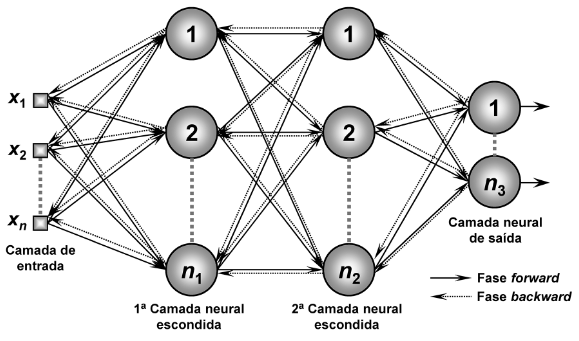
\includegraphics[scale=0.6]{backpropagation.png}\\
            {\footnotesize Fonte: Da Silva (2016).}\
            \label{fig:fluxo-backpropagation}
        \end{figure}
        \citeonline{grus2021} apresenta o funcionamento padrão do treinamento de uma rede neural utilizando o algoritmo 
        de backpropagation como método de ajuste dos pesos. Considera-se que a rede possui \( n\),  os quais são 
        ajustados de acordo com o seguinte procedimento:
        \begin{enumerate}
            \item Realiza-se o \emph{feed-forward}, em que as entradas são processadas para produzir as saídas de todos os neurônios;
            \item Como o algoritmo é supervisionado, os valores esperados das saídas são conhecidos. Assim, calcula-se uma função de perda, geralmente definida como a soma dos erros quadráticos entre as saídas reais e as esperadas;
            \item O gradiente dessa função de perda é calculado em relação aos pesos dos neurônios de saída;
            \item Os gradientes e os erros são propagados para trás com o objetivo de calcular os gradientes associados aos pesos dos neurônios ocultos;
            \item Atualizam-se os pesos aplicando um passo em direção ao gradiente descendente, controlado por um parâmetro denominado learning rate (taxa de aprendizagem).
        \end{enumerate}